\documentclass[12pt]{article}
\usepackage[english]{babel}
\usepackage[utf8x]{inputenc}
\usepackage{amsmath}
\usepackage{graphicx}
\usepackage[colorinlistoftodos]{todonotes}
\usepackage[margin=1in]{geometry}

\begin{document}
	
	\begin{titlepage}
		\newcommand{\HRule}{\noindent\rule{6.5in}{1pt}} % Defines a new command for the horizontal lines, change thickness here
		
		\centering
		
		\textsc{\Large Intro to Artificial Intelligence}\\[.75cm]
		
		\noindent\rule{6.5in}{1.5pt}\\[.75cm]
		{ \huge \bfseries Assignment 2}\\[.4cm]
		{ \large \bfseries Search Problems in AI}\\[.2cm]
		\noindent\rule{6.5in}{1.5pt}\\[1cm]
		
		
		\begin{minipage}{0.4\textwidth}
			\begin{flushleft} \large
				\emph{Authors:}\\
				Brian \textsc{Lin} \\
				Samuel \textsc{Yang}
			\end{flushleft}
		\end{minipage}
		~
		\begin{minipage}{0.4\textwidth}
			\begin{flushright} \large
				\emph{Supervisor:} \\
				Dr. Abdeslam  \textsc{Boularias} % Supervisor's Name
			\end{flushright}
		\end{minipage}\\[2cm]

		
\includegraphics[width=200pt,height=200pt]{RutgersLogo.png}\\[1.5cm]
		\textsc{\Large Rutgers State University of New Jersey}\\[1cm]
		{\large \today}\\[2cm]
		
		\vfill % Fill the rest of the page with whitespace
		
	\end{titlepage}
	
	\section*{Problem 1}
		The order of expanded cities is (city, f(city), g(city), h(city)): \\ \\
		(Lugoj, 244,0,244) \\ 
		(Mehadia,311,70,241) \\
		(Drobeta,387,145,242) \\
		(Craiova,425,265,160) \\
		(Timisoara,440,111,329) \\
		(Pitesi,503,403,100) \\
		(Bucharest,504,504,0)
		
	\section*{Problem 2}
		\begin{figure}[!htb]
			\centering
			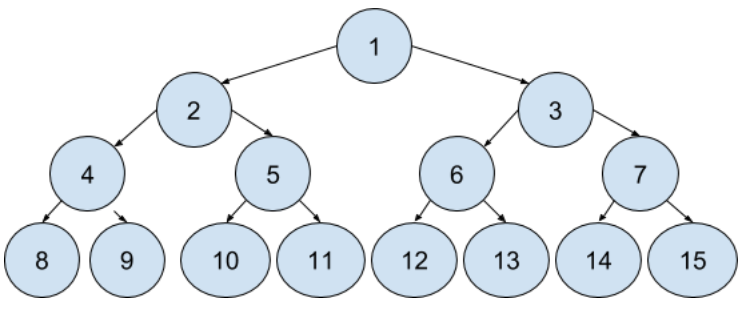
\includegraphics[width=.5\textwidth]{Question2.png}
		\end{figure}
		\subsection*{Part A}
			BFS: States Visited: 1, 2, 3, 4, 5, 6, 7, 8, 9, 10, 11, stops at 11 \\
			Depth Limited Search By 3: 1, 2, 4, 8, 9, 5, 10, 11, stops at 11 \\
			Iterative Deepening Search: \\
			Iteration limit = 0:1 \\
			Iteration limit = 1:1, 2, 3 \\
			Iteration limit = 2:1, 2, 4, 5, 3, 6, 7 \\
			Iteration limit = 3:1, 2, 4, 8, 9, 5, 10, 11 stops at 11
		\subsection*{Part B}
			Looking at the tree, if we were to run a bfs from the goal state 11, the only branch it could go to is 5, then moving back from 5, the only branch is to go to 2. This indicates that going in the reverse direction has a branching factor of 1, which would be very useful because it produces a more focused search compared to the branching factor of 2 in the forward direction. \\
			Forward Expansion:1,2,3 \\
			Reverse Expansion:11,5,2 \\
			Stop after 3 expansions, because they have now intersected, with the path of going from 1,2,5,11
		
	\section*{Problem 3}
		\subsection*{Part A}
			Yes, BFS is a special case of Uniform cost search. In the case where the cost to go to every child is a constant (every step to the next child is equal), then uniform cost operates like a breadth-first search. This is because uniform cost search will choose a child with the lowest g value or cost from the start, but if all the costs are the same, then it will just expand whatever children it has at each level, which is a BFS.
		\subsection*{Part B}
			Yes. In a best first tree search, it operates much in the same way of a DFS, but it expands the states with the lowest cost or f value. Like with Part A, using specific f values will lead to the desired result. In this case, we want to expand downwards first before exploring the other children. This can be done by having the f value equal to negative of the depth. This will result in a best first tree which will expand a child, then expand its child because the children will always have lower f values thus becoming a DFS.
		\subsection*{Part C}
			Yes, A* and Uniform Cost Search both operate by having an open list of states, and choosing the one with the least f value. In Uniform Cost Search, the f value is just the g value (total cost from the start) whereas A* f value is g value plus the heuristic. If for some reason the heuristic was always 0, then A* would operate exactly like a Uniform Cost Search.
			
	\section*{Problem 4}
		To be admissible, the heuristic must never overestimate the cost to reach the goal. To be consistent, for every state, the heuristic of that state should be less than the heuristic of it’s child plus the cost of going to the child. In order to prove admissibility, we must say that some h(n) is less than or equal to the optimal solution o(n). To prove this we will use induction: \\
		
		\noindent Assume: h(n) < o(n) for any state n \\
		Base: If we’re already at the goal, then h(n) = 0 <= o(n) \\
		
		\noindent Inductive Step: If we are at state n, not the goal state, then there should exist some successor to the current state n’ that will be on the optimal path o(n). Since we are assuming consistency, \\
		
		\noindent h(n) <= c(n,a,n’) + h(n’) \\
		
		\noindent If we are to assume n’ is on the optimal path, then plugging in the inductive hypothesis gives us \\
		
		\noindent h(n) <= c(n,a,n’) + o(n’), where c(n,a,n’) + o(n’) = o(n), so h(n) <= o(n) and consistency implies admissibility.
		
		\begin{figure}[!htb]
			\centering
			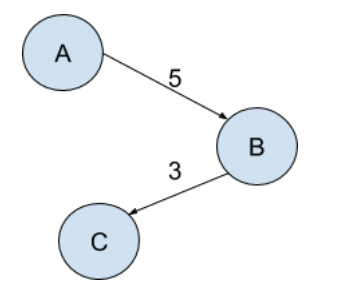
\includegraphics[width=.5\textwidth]{Question4.png}
			\caption{An example scenario}
		\end{figure}
		\noindent For this example, let’s say C is the goal node. That means the optimal path o(C) = 0, o(B) = 3, and o(A) = 8. In order to be admissible, the heuristic for h(C) = 0, h(B) <= 3, and h(A) <= 8. If we assign some arbitrary values to the heuristic, we could have h(C) = 0, h(B) = 1, and h(A) = 8. If this were consistent, then h(A) <= h(B) + cost(A to B). Plugging in we have 8 <= 1+5, or 8 <= 6, which is not a true statement, so it is not consistent. Thus we have heuristics which are admissible but not consistent.
		
	\section*{Problem 5}
		It’s a good idea to choose the variable that is the most constrained in a CSP because it is likely the one that has the most constrained domain will have few solutions to work with in the end. If we were to choose a less constrained heuristic than the most constrained, a likely scenario would be we would further constrain the domain in the most constrained domain until there is nothing left, or there is no workable solution. This would force us to backtrack and expend more resources on finding possibilities that do work. By using variables that are the least constrained, we have more possible paths that can lead to a solution and lessen the amount of backtracking needed.
		
	\section*{Problem 6}
		\subsection*{Part A}
			The optimal play for the max player is to choose the right branch (branch C). If we go to the left, we’ll end up with 3, because the min player will choose 3. In the right branch, there are three options, one of which is 4 for H. Working all the way from the bottom, at node I, it is the MIN players turn, who would naturally choose 0 over 7. Then at node F, the MAX Player has the option of 0 or 5, which should result in 5. At node G, the MAX Player would choose 8. So the MIN player has three options at node C: 5(F), 8(G), or 4(H) where he will choose 4. So the resulting options for the MAX player is to go B, which will result in 3, or go C, which will result in 4. The optimal solution for maximizing is C, so the MAX player should go the right.
		\subsection*{Part B} 
			\begin{figure}[!htb]
				\centering
				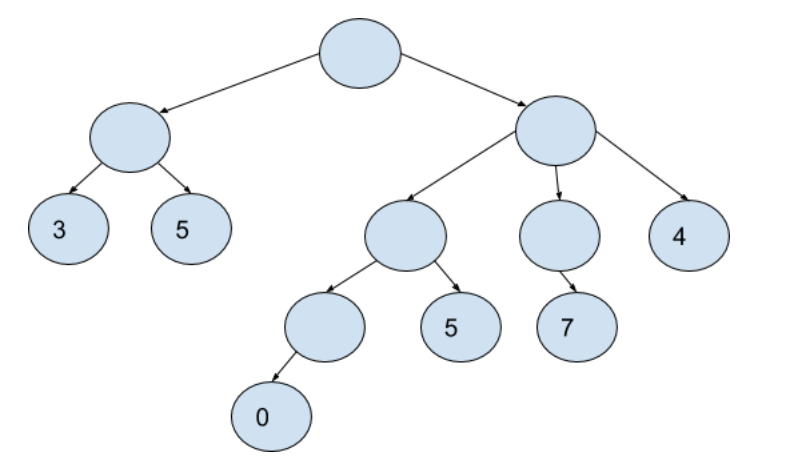
\includegraphics[width=.5\textwidth]{Question6a.png}
				\caption{Pruning from left to right}
			\end{figure}
		\subsection*{Part C}
			\begin{figure}[!htb]
				\centering
				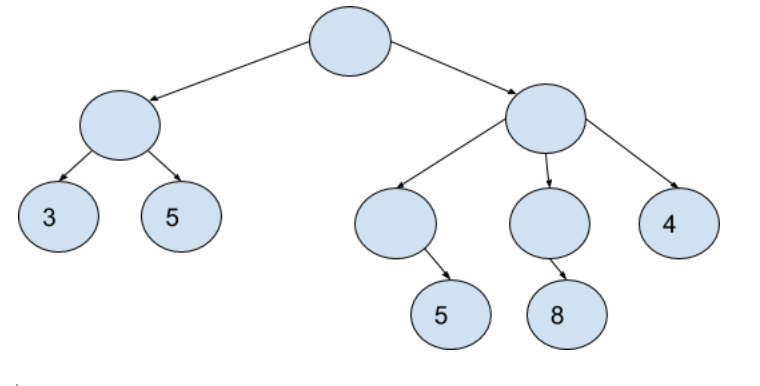
\includegraphics[width=.5\textwidth]{Question6b.png}
				\caption{Pruning from right to left}
			\end{figure}
			It makes sense that the tree would look different because our updated alpha beta values become different as we have different starting information to work with. As we progress with the pruning, this will lead to differences in the pruning done and ultimately a different looking tree between part B and part C.
			
	\section*{Problem 7}
		\subsection*{Admissible h1, h2}
			$h(n) = min\{h_1(n), h_2(n)\}$ \\
			min(h1,h2) is admissible, because both should be less than the optimal solution\\ \\
			$h(n) = wh_1(n) + (1-w)h_2(n)$, where 0 $\leq$ $w$ $\leq$ 1 \\  
			h(n) = wh1(n) + (1 − w)h2(n) is admissible because, this acts like a weighted average between both heuristics, where the highest value that can be obtained is max(h1,h2),  the lowest is min(h1, h2), and typically operates in a value in between h1 and h2 which is still admissible. \\ \\
			$h(n) = max\{h_1(n), h_2(n)\}$ \\
			max(h1,h2) is admissible, also because both should be less
			
		\subsection*{Consistent h1, h2}			
		$h(n) = min\{h_1(n), h_2(n)\}$ \\
		min(h1,h2) is consistent, because regardless of which is chosen, both are consistent, the resulting answer should be consistent.\\ \\
		$h(n) = wh_1(n) + (1-w)h_2(n)$, where 0 $\leq$ $w$ $\leq$ 1 \\  
		 h(n) = wh1(n) + (1 − w)h2(n) is consistent because h is now any range of values between min(h1,h2) and max(h1,h2). \\ \\
		$h(n) = max\{h_1(n), h_2(n)\}$ \\
		max(h1,h2) is consistent, also because both h1 and h2 are consistent, so either or should give a consistent heuristic.
	
	\section*{Problem 8}
		\subsection*{Part A}
		Simulated annealing is not necessary if we are dealing with no global maxima, where finding the global maximum is mute so normal hill climbing will produce a faster result.
		\subsection*{Part B}
		For randomly guessing to work just as well as simulated annealing, your model would have to be completely without any structure, where the model simply doesn’t have any geometry for hill climbing to figure out where to go next because the algorithm wouldn’t be able to tell if it getting further or closer to the global maximum.
		\subsection*{Part C}
		Ideally for simulated annealing, you would have some definite geometry that flows and provides information on which general direction is better or worse. In addition, one where we have several local maxima scattered about.
		\subsection*{Part D}
		You can keep a running value for the maximum as you run the simulated annealing. Everytime a higher value comes in, we replace it and keep that as our max, while keeping a record of the state itself. In the case that the simulated annealing ends in a slightly lower position, we always have the record of being in that higher state which is more likely to be the global maximum.
		\subsection*{Part E}
	
	\section*{Problem 9}
		\begin{figure}[!htb]
			\centering
			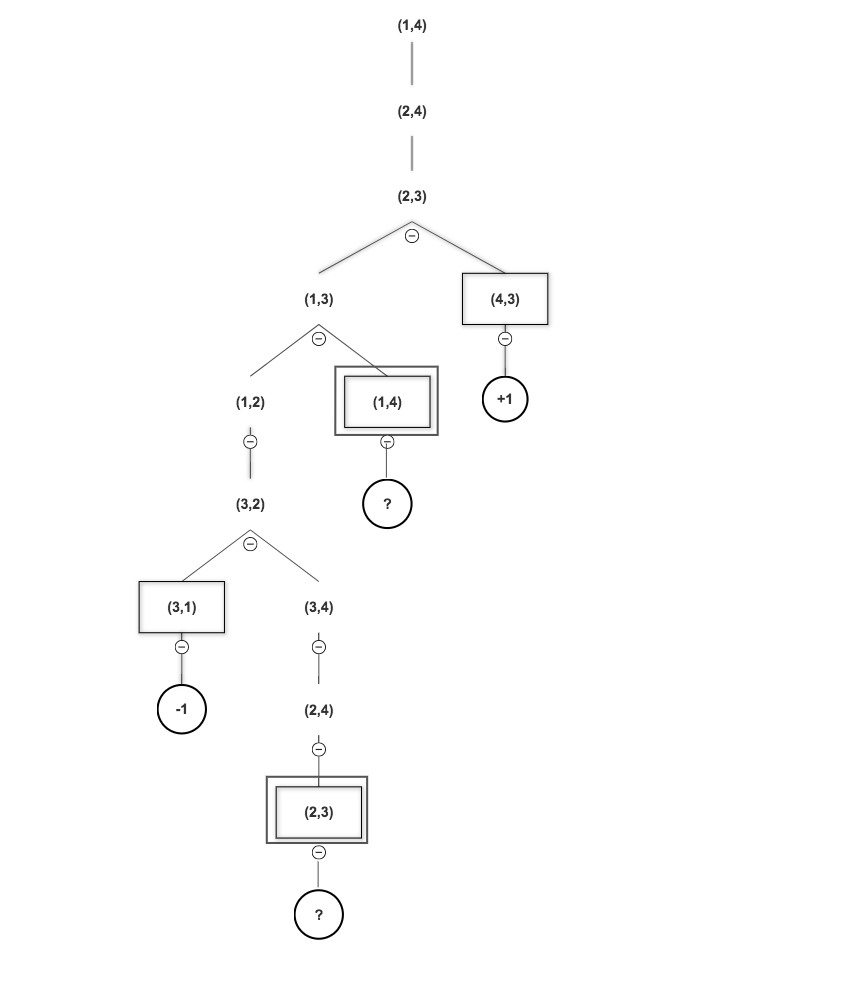
\includegraphics[width=.8\textwidth]{Question9.png}

		\end{figure}  
\end{document}